%% =======================================================
%% Actividad 3: Tipos de variables y su manipulación computacional
%%
%% Compilar desde actividades/: ./compilar.sh act03
%% =======================================================

%% ---- CONFIGURACIÓN ------------------------

\documentclass[11pt,letterpaper]{article}

\usepackage[indice]{tecnm}
\usepackage[T1]{fontenc}
\usepackage{amsmath, amssymb}
\usepackage{xcolor}
\usepackage[most]{tcolorbox} % Carga tcolorbox con soporte para listings y saltos de página
\tcbuselibrary{listings, skins, breakable}
\setlength{\emergencystretch}{3em} % Evita líneas desbordadas por palabras en \texttt

% Paleta de colores (estilo GitHub Light / VS Code)
\definecolor{codebg}{HTML}{F8F9FA}       % Fondo del código
\definecolor{codehead}{HTML}{E9ECEF}     % Fondo de la barra de título
\definecolor{codeborder}{HTML}{CED4DA}   % Borde de la tarjeta
\definecolor{codetitle}{HTML}{212529}    % Texto del título
\definecolor{codekw}{HTML}{0550AE}       % Palabras clave (import, def, for...)
\definecolor{codefunc}{HTML}{8250DF}     % Funciones y métodos (describe, groupby...)
\definecolor{codestr}{HTML}{0A3069}      % Strings
\definecolor{codecomm}{HTML}{6E7781}     % Comentarios
\definecolor{codenum}{HTML}{8C959F}      % Números de línea
\definecolor{codeid}{HTML}{24292F}       % Texto general

% Configuración base de listings
\lstdefinestyle{pythonestilo}{
  language=Python,
  basicstyle=\ttfamily\footnotesize\color{codeid},
  keywordstyle=\color{codekw}\bfseries,
  keywordstyle=[2]\color{codefunc}, % Estilo secundario para métodos de datos
  stringstyle=\color{teal!80!black},
  commentstyle=\color{codecomm}\itshape,
  morekeywords={as, True, False, None, with, yield, lambda},
  morekeywords=[2]{read_csv, head, tail, info, describe, groupby, mean, value_counts, to_csv, print, len, range, DataFrame, Categorical, Series, get_dummies, set_index, astype, MinMaxScaler, fit_transform, ravel, min, max, sum, cumsum, to_frame, tolist, all},
  numbers=left,
  numberstyle=\tiny\ttfamily\color{codenum},
  stepnumber=1,
  numbersep=10pt,
  showstringspaces=false,
  morestring=[b]{"""},
  tabsize=4,
  breaklines=true,
  breakatwhitespace=true,
  columns=flexible,
  keepspaces=true,
  literate=
    {á}{{\'a}}1 {é}{{\'e}}1 {í}{{\'i}}1 {ó}{{\'o}}1 {ú}{{\'u}}1
    {Á}{{\'A}}1 {É}{{\'E}}1 {Í}{{\'I}}1 {Ó}{{\'O}}1 {Ú}{{\'U}}1
    {ñ}{{\~n}}1 {Ñ}{{\~N}}1 {¿}{{?`}}1 {¡}{{!`}}1
}

% Definición del entorno personalizado \begin{codigo}{Título}{etiqueta}
% \newtcblisting[auto counter, number within=section]{codigo}[2][]{
\newtcblisting[auto counter]{codigo}[2][]{
  listing only,
  breakable,                    % Permite que el bloque se divida si pasa de página
  enhanced,
  colback=codebg,
  colframe=codeborder,
  colbacktitle=codehead,
  coltitle=codetitle,
  fonttitle=\bfseries\small\sffamily,
  boxrule=0.6pt,
  arc=4pt,                      % Bordes redondeados
  left=20pt,                    % Espacio izquierdo para los números de línea
  right=8pt,
  top=6pt,
  bottom=6pt,
  toptitle=4pt,
  bottomtitle=4pt,
  before skip=12pt,
  after skip=12pt,
  listing options={style=pythonestilo},
  title={Código \thetcbcounter: #2},
  #1
}

% Paleta para salida de consola (estilo terminal limpia)
\definecolor{termbg}{HTML}{212529}      % Fondo oscuro tipo terminal
\definecolor{termhead}{HTML}{343A40}    % Barra superior
\definecolor{termtext}{HTML}{F8F9FA}    % Texto claro de alta legibilidad
\definecolor{termborder}{HTML}{495057}  % Borde

% Entorno \begin{consola}[label=out:iris]{Título}
\newtcblisting[auto counter]{consola}[2][]{
  listing only,
  breakable,
  colback=termbg,
  colframe=termborder,
  colbacktitle=termhead,
  coltitle=termtext,
  colupper=termtext,
  fonttitle=\bfseries\small\sffamily,
  boxrule=0.6pt,
  arc=4pt,
  left=8pt,
  right=8pt,
  top=6pt,
  bottom=6pt,
  toptitle=4pt,
  bottomtitle=4pt,
  before skip=12pt,
  after skip=12pt,
  listing options={
    basicstyle=\ttfamily\scriptsize\color{termtext}, % \scriptsize evita que las tablas de Pandas se partan de línea
    breaklines=true,
    columns=fixed,        % Mantiene alineadas las columnas de Pandas
    keepspaces=true,
    showstringspaces=false,
    literate=
      {á}{{\'a}}1 {é}{{\'e}}1 {í}{{\'i}}1 {ó}{{\'o}}1 {ú}{{\'u}}1
      {Á}{{\'A}}1 {É}{{\'E}}1 {Í}{{\'I}}1 {Ó}{{\'O}}1 {Ú}{{\'U}}1
      {ñ}{{\~n}}1 {Ñ}{{\~N}}1 {¿}{{?`}}1
  },
  title={Salida \thetcbcounter: #2},
  #1
}

%% ---- DATOS DE LA MATERIA ------------------------

\materia{Modelos Estadísticos para el Aprendizaje \\ Automático y Ciencia de Datos}
\actividad{Tema 1.2
Tipos de Variables en un Conjunto de Datos y su Manipulación Computacional \\ Actividad 3 - Ejercicios Prácticos}

\profesor{Dr. José Ismael Ojeda Campaña}
%\fecha{15 de octubre de 2026}    % opcional; por defecto es la fecha de hoy

\begin{document}
\portada
\indicegeneral

%% ---- CONTENIDO ---------------------------------

\section{Introducción}

Antes de analizar un conjunto de datos o de entrenar un modelo de aprendizaje automático es necesario saber qué tipo de información contiene cada variable. No es lo mismo una variable que nombra una categoría, como el color de ojos, que una que mide una cantidad, como la altura. El tipo de cada variable determina qué operaciones tienen sentido sobre ella, qué resúmenes estadísticos se le pueden aplicar y cómo debe transformarse para que un algoritmo pueda procesarla \parencite{tecnm2026_documento_fuente,bruce2020}.

En este documento se resuelven los ejercicios prácticos del tema 1.2 a partir de un pequeño conjunto de datos de cinco personas. Primero se clasifican sus variables en cualitativas (nominales u ordinales) y cuantitativas (discretas o continuas). Después se aplican en Python las técnicas de manipulación computacional presentadas en el tema: la codificación One-Hot de una variable nominal con \texttt{pandas}, la normalización Min-Max de una variable continua con \texttt{scikit-learn} y el análisis de frecuencias de una variable ordinal con \texttt{value\_counts()}.

\section{Marco conceptual}

\subsection{Variables aleatorias}

Una variable aleatoria traslada los resultados de un experimento, que pertenecen a un espacio muestral abstracto $\Omega$, al conjunto de los números reales, donde es más sencillo trabajar. Formalmente, una variable aleatoria es una función $X : \Omega \to \mathbb{R}$ tal que, para cualquier conjunto de Borel $B$, el conjunto $X^{-1}(B)$ es un suceso. Al usar una variable aleatoria se genera una nueva forma de medir probabilidades sobre $\mathbb{R}$, llamada distribución o ley de probabilidad de $X$ \parencite{tecnm2026_documento_fuente}.

Como manipular toda la distribución puede ser complejo, se usa la función de distribución acumulada:
\begin{equation}
    F_X(x) = P(X \leq x),
\end{equation}
que siempre es creciente, es continua por la derecha y tiende a 0 cuando $x \to -\infty$ y a 1 cuando $x \to +\infty$ \parencite{tecnm2026_documento_fuente}.

Según los valores que puede tomar, una variable aleatoria es:

\begin{itemize}
    \item \textbf{Discreta}, si solo puede tomar valores de un conjunto finito o contable $D$, de modo que $P(X \in D) = 1$. Sus valores suelen ser enteros y se obtienen al contar, como el número de hijos en una familia o la edad medida en años completos \parencite{tecnm2026_documento_fuente}.
    \item \textbf{Continua}, si puede tomar infinitos valores dentro de un intervalo, como el peso, la altura o la temperatura. Tiene una función de densidad $f(x)$, y las probabilidades se calculan como áreas bajo esa curva \parencite{tecnm2026_documento_fuente}:
    \begin{equation}
        P(a < X \leq b) = \int_a^b f(x)\, dx.
    \end{equation}
\end{itemize}

\subsection{Tipos de variables en un conjunto de datos}

En la práctica, las variables de un conjunto de datos se clasifican en dos grandes grupos, cada uno con dos subtipos \parencite{tecnm2026_documento_fuente,bruce2020}:

\begin{itemize}
    \item \textbf{Cualitativas o categóricas.} Representan categorías o grupos.
    \begin{itemize}
        \item \textbf{Nominales:} no tienen un orden inherente. Por ejemplo, el color de ojos: azul, verde o marrón.
        \item \textbf{Ordinales:} tienen un orden, pero las diferencias entre categorías no son cuantificables. Por ejemplo, una escala de satisfacción: muy insatisfecho, insatisfecho, neutral.
    \end{itemize}
    \item \textbf{Cuantitativas o numéricas.} Representan cantidades numéricas.
    \begin{itemize}
        \item \textbf{Discretas:} toman un número limitado de valores enteros. Por ejemplo, el número de hijos.
        \item \textbf{Continuas:} pueden tomar cualquier valor dentro de un rango. Por ejemplo, la altura o el peso.
    \end{itemize}
\end{itemize}

La Figura~\ref{fig:tipos} resume esta clasificación.

\begin{figure}[htbp]
\centering
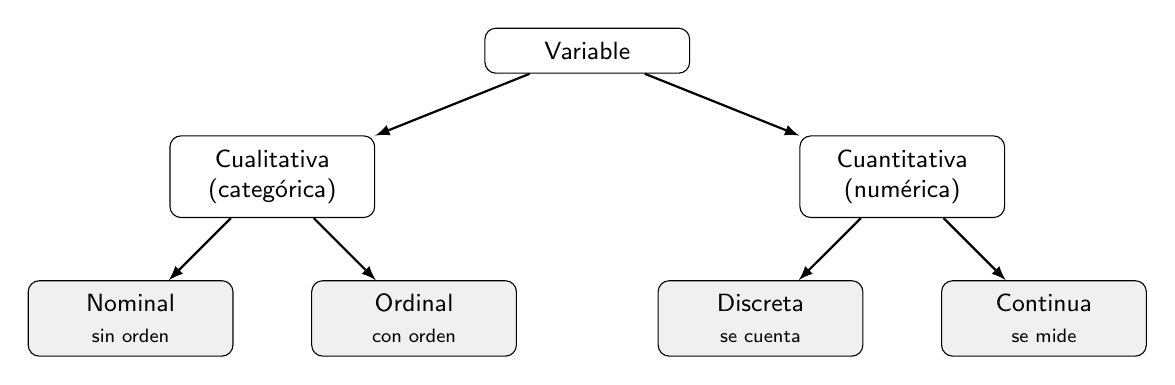
\begin{tikzpicture}[
  caja/.style={draw, rounded corners, align=center, font=\small\sffamily, inner sep=5pt, minimum width=26mm},
  hoja/.style={caja, fill=gray!12},
  flecha/.style={-latex, thick},
]
\node[caja] (var) at (0, 0) {Variable};
\node[caja] (cual) at (-4, -1.6) {Cualitativa\\(categórica)};
\node[caja] (cuan) at (4, -1.6) {Cuantitativa\\(numérica)};
\node[hoja] (nom) at (-5.8, -3.4) {Nominal\\\scriptsize sin orden};
\node[hoja] (ord) at (-2.2, -3.4) {Ordinal\\\scriptsize con orden};
\node[hoja] (dis) at (2.2, -3.4) {Discreta\\\scriptsize se cuenta};
\node[hoja] (con) at (5.8, -3.4) {Continua\\\scriptsize se mide};
\draw[flecha] (var) -- (cual);
\draw[flecha] (var) -- (cuan);
\draw[flecha] (cual) -- (nom);
\draw[flecha] (cual) -- (ord);
\draw[flecha] (cuan) -- (dis);
\draw[flecha] (cuan) -- (con);
\end{tikzpicture}
\caption{Clasificación de las variables de un conjunto de datos según el documento fuente \parencite{tecnm2026_documento_fuente}.}
\label{fig:tipos}
\end{figure}

\subsection{Manipulación computacional de variables}

Muchos algoritmos de aprendizaje automático solo operan con números, y otros son sensibles a la escala de las variables. Por eso, en la práctica es necesario codificar o transformar las variables, especialmente las cualitativas \parencite{tecnm2026_documento_fuente}. Dos técnicas comunes son:

\begin{itemize}
    \item \textbf{Codificación One-Hot.} Convierte una variable categórica en variables binarias. Se crea una nueva columna por cada categoría única, que vale 1 (o \texttt{True}) si la fila pertenece a esa categoría y 0 (o \texttt{False}) si no. En \texttt{pandas} se realiza con la función \texttt{pd.get\_dummies()} \parencite{tecnm2026_documento_fuente,bruce2020}.
    \item \textbf{Normalización Min-Max.} Escala una variable cuantitativa al rango de 0 a 1 mediante la fórmula
    \begin{equation}
        X_{\text{norm}} = \frac{X - \min(X)}{\max(X) - \min(X)}.
        \label{eq:minmax}
    \end{equation}
    En \texttt{scikit-learn}, la clase \texttt{MinMaxScaler} calcula el mínimo y el máximo con \texttt{.fit()} y aplica la fórmula con \texttt{.transform()} \parencite{tecnm2026_documento_fuente}.
\end{itemize}

Para las variables cualitativas, además, el resumen más natural es la tabla de frecuencias, que cuenta cuántas veces aparece cada categoría \parencite{guisande2013}. En \texttt{pandas} se obtiene con el método \texttt{value\_counts()}.

\section{Descripción de la actividad}

\textbf{Objetivo:} Identificar los tipos de variables de un conjunto de datos y aplicar en Python las técnicas de codificación, normalización y análisis de frecuencia correspondientes a cada tipo.

La actividad se basa en el conjunto de datos de la Tabla~\ref{tab:datos}, que describe a cinco personas mediante cinco variables \parencite{tecnm2026_documento_fuente}.

\begin{table}[htbp]
\centering
\caption{Conjunto de datos de los ejercicios prácticos \parencite{tecnm2026_documento_fuente}.}
\label{tab:datos}
\begin{tabular}{cccccc}
\hline
\textbf{ID} & \textbf{Color de Ojos} & \textbf{Satisfacción} & \textbf{Edad} & \textbf{Número de Hijos} & \textbf{Altura (cm)} \\
\hline
1 & Azul   & Alta  & 25 & 2 & 170 \\
2 & Verde  & Baja  & 34 & 1 & 165 \\
3 & Marrón & Media & 42 & 3 & 180 \\
4 & Azul   & Alta  & 28 & 0 & 160 \\
5 & Marrón & Baja  & 37 & 4 & 175 \\
\hline
\end{tabular}
\end{table}

Sobre este conjunto se resolvieron los siguientes ejercicios:

\begin{description}
    \item[Ejercicio 1.1: Identificación de tipos de variables.] Clasificar cada variable como cualitativa (nominal u ordinal) o cuantitativa (discreta o continua).
    \item[Ejercicio 1.2: Codificación One-Hot en Python.] Codificar la variable \textit{Color de Ojos} en formato One-Hot y explicar la salida y el significado de las columnas generadas.
    \item[Ejercicio 1.3: Normalización de datos cuantitativos.] Normalizar la variable \textit{Altura} al rango de 0 a 1 con la fórmula~\eqref{eq:minmax} e indicar los valores obtenidos.
    \item[Ejercicio 1.4: Análisis de frecuencia.] Calcular la frecuencia de cada categoría de la variable \textit{Satisfacción} con \texttt{value\_counts()}.
\end{description}

\section{Desarrollo}

Los cuatro ejercicios se resolvieron en un solo script que usa \texttt{pandas} y \texttt{scikit-learn}. Para los Ejercicios 1.2 a 1.4 se completó el código base del cuaderno de trabajo en los lugares indicados por sus comentarios. Además, se agregaron extensiones que comprueban o amplían cada resultado. El script se presenta a continuación en cuatro partes, una por ejercicio. El cuaderno interactivo puede consultarse en Google Colab:

\begin{center}
    \url{https://colab.research.google.com/drive/1AA0cvaVJ1gLNoYwMfM8YCpF7krnsGAWF?usp=sharing}
\end{center}

\subsection{Ejercicio 1.1: Identificación de tipos de variables}

El conjunto de datos se construyó como un \texttt{DataFrame} con la columna \texttt{ID} como índice, ya que solo identifica a cada persona y no es una variable de análisis. La clasificación de las variables se registró en una tabla. Como extensión, cada variable se convirtió al tipo de dato de \texttt{pandas} que mejor representa su naturaleza:

\begin{itemize}
    \item \textit{Color de Ojos} se convirtió al tipo \texttt{category}, que almacena las categorías sin orden.
    \item \textit{Satisfacción} se convirtió a un \texttt{Categorical} ordenado (\texttt{ordered=True}) con el orden $\text{Baja} < \text{Media} < \text{Alta}$. Esto permite hacer comparaciones como \texttt{>= 'Media'}, que no tendrían sentido en una variable nominal.
    \item \textit{Edad} y \textit{Número de Hijos} se mantuvieron como enteros (\texttt{int64}).
    \item \textit{Altura} se convirtió a punto flotante (\texttt{float64}), porque es una medida que puede tomar cualquier valor real.
\end{itemize}

\begin{codigo}[label=cod:ej11]{Ejercicio 1.1: tipos de variables}
import pandas as pd
from sklearn.preprocessing import MinMaxScaler

# Conjunto de datos del Ejercicio 1.1
df = pd.DataFrame({
    'ID': [1, 2, 3, 4, 5],
    'Color de Ojos': ['Azul', 'Verde', 'Marrón', 'Azul', 'Marrón'],
    'Satisfacción': ['Alta', 'Baja', 'Media', 'Alta', 'Baja'],
    'Edad': [25, 34, 42, 28, 37],
    'Número de Hijos': [2, 1, 3, 0, 4],
    'Altura (cm)': [170, 165, 180, 160, 175],
}).set_index('ID')

clasificacion = pd.DataFrame({
    'Tipo': ['Cualitativa', 'Cualitativa', 'Cuantitativa', 'Cuantitativa', 'Cuantitativa'],
    'Subtipo': ['Nominal', 'Ordinal', 'Discreta', 'Discreta', 'Continua'],
}, index=df.columns)

# Representación computacional de cada tipo en pandas
df['Color de Ojos'] = df['Color de Ojos'].astype('category')
df['Satisfacción'] = pd.Categorical(df['Satisfacción'],
                                    categories=['Baja', 'Media', 'Alta'], ordered=True)
df['Altura (cm)'] = df['Altura (cm)'].astype(float)
clasificacion['dtype en pandas'] = df.dtypes.astype(str)

print("=== Ejercicio 1.1: tipos de variables ===")
print(df)
print()
print(clasificacion)

# Una variable ordinal admite comparaciones de orden, una nominal no
print("\nSatisfacción >= 'Media':")
print(df['Satisfacción'] >= 'Media')
\end{codigo}

\subsection{Ejercicio 1.2: Codificación One-Hot}

Se completó el código base creando el \texttt{DataFrame} a partir del diccionario \texttt{data} y aplicando \texttt{pd.get\_dummies()} sobre la columna \textit{Color de Ojos}. Como extensión, se repitió la codificación con \texttt{dtype=int} para obtener 0 y 1 en lugar de \texttt{False} y \texttt{True}. También se comprobó que la suma de cada fila es 1, es decir, que cada persona pertenece exactamente a una categoría.

\begin{codigo}[label=cod:ej12]{Ejercicio 1.2: codificación One-Hot}
data = {
    'Color de Ojos': ['Azul', 'Verde', 'Marrón', 'Azul', 'Marrón']
}

# Crear un dataframe
df_ojos = pd.DataFrame(data)

# Realizar la codificación One-Hot
df_one_hot = pd.get_dummies(df_ojos, columns=['Color de Ojos'])

print("\n=== Ejercicio 1.2: codificación One-Hot ===")
print(df_one_hot)

# Misma codificación con 0 y 1 en lugar de False y True
df_one_hot_01 = pd.get_dummies(df_ojos, columns=['Color de Ojos'], dtype=int)
print("\nCon dtype=int:")
print(df_one_hot_01)

# Cada fila tiene exactamente un 1: la categoría a la que pertenece
print("\nSuma por fila:", df_one_hot_01.sum(axis=1).tolist())
\end{codigo}

\subsection{Ejercicio 1.3: Normalización Min-Max}

Se completó el código base creando el objeto \texttt{MinMaxScaler} y aplicando \texttt{fit\_transform()} a la variable \textit{Altura}. Como \texttt{scikit-learn} espera una matriz con una fila por observación y una columna por variable, la lista se colocó primero en un \texttt{DataFrame} de una columna. Como extensión, los valores también se calcularon directamente con la fórmula~\eqref{eq:minmax} y se compararon con los de \texttt{MinMaxScaler}.

\begin{codigo}[label=cod:ej13]{Ejercicio 1.3: normalización de Altura}
altura = [170, 165, 180, 160, 175]

# Crear el objeto scaler
scaler = MinMaxScaler()

# Normalizar los datos (MinMaxScaler espera una matriz de n filas x 1 columna)
df_altura = pd.DataFrame({'Altura (cm)': altura})
df_altura['Normalizada'] = scaler.fit_transform(df_altura[['Altura (cm)']]).ravel()

# Verificación con la fórmula (1.8): (X - min) / (max - min)
minimo, maximo = min(altura), max(altura)
df_altura['Fórmula (1.8)'] = [(x - minimo) / (maximo - minimo) for x in altura]

print("\n=== Ejercicio 1.3: normalización de Altura ===")
print(f"Mínimo = {scaler.data_min_[0]:.0f}, Máximo = {scaler.data_max_[0]:.0f}")
print(df_altura)
print("¿Coinciden MinMaxScaler y la fórmula?",
      (df_altura['Normalizada'] == df_altura['Fórmula (1.8)']).all())
\end{codigo}

\subsection{Ejercicio 1.4: Análisis de frecuencia}

Se completó el código base creando el \texttt{DataFrame} con la lista \texttt{satisfaccion} y calculando las frecuencias con \texttt{value\_counts()}. Este método ordena las categorías de mayor a menor frecuencia, lo que no respeta el orden natural de una variable ordinal. Como extensión, se construyó una tabla de frecuencias completa con las categorías en el orden $\text{Baja} < \text{Media} < \text{Alta}$. La tabla incluye la frecuencia absoluta, la relativa (proporción del total), la acumulada y la relativa acumulada. Las frecuencias acumuladas solo tienen sentido en variables cuyas categorías tienen un orden.

\begin{codigo}[label=cod:ej14]{Ejercicio 1.4: frecuencias de Satisfacción}
satisfaccion = ['Alta', 'Baja', 'Media', 'Alta', 'Baja']

# Crear un dataframe
df_satisfaccion = pd.DataFrame({'Satisfacción': satisfaccion})

# Calcular la frecuencia de cada categoría
frecuencias = df_satisfaccion['Satisfacción'].value_counts()

print("\n=== Ejercicio 1.4: frecuencia de Satisfacción ===")
print(frecuencias)

# Tabla de frecuencias en el orden natural de la variable ordinal
orden = pd.Categorical(satisfaccion, categories=['Baja', 'Media', 'Alta'], ordered=True)
tabla = pd.Series(orden).value_counts(sort=False).to_frame('Frecuencia')
tabla['Relativa'] = tabla['Frecuencia'] / tabla['Frecuencia'].sum()
tabla['Acumulada'] = tabla['Frecuencia'].cumsum()
tabla['Relativa acumulada'] = tabla['Relativa'].cumsum()
tabla.index.name = 'Satisfacción'

print("\nTabla de frecuencias ordenada:")
print(tabla)
\end{codigo}

\section{Resultados}

\subsection{Ejercicio 1.1: Identificación de tipos de variables}

\begin{consola}[label=out:ej11]{Ejecución de \texttt{act03.py}: Ejercicio 1.1}
=== Ejercicio 1.1: tipos de variables ===
   Color de Ojos Satisfacción  Edad  Número de Hijos  Altura (cm)
ID
1           Azul         Alta    25                2        170.0
2          Verde         Baja    34                1        165.0
3         Marrón        Media    42                3        180.0
4           Azul         Alta    28                0        160.0
5         Marrón         Baja    37                4        175.0

                         Tipo   Subtipo dtype en pandas
Color de Ojos     Cualitativa   Nominal        category
Satisfacción      Cualitativa   Ordinal        category
Edad             Cuantitativa  Discreta           int64
Número de Hijos  Cuantitativa  Discreta           int64
Altura (cm)      Cuantitativa  Continua         float64

Satisfacción >= 'Media':
ID
1     True
2    False
3     True
4     True
5    False
Name: Satisfacción, dtype: bool
\end{consola}

La Tabla~\ref{tab:clasificacion} resume la clasificación obtenida. A continuación se responden las preguntas del ejercicio.

\begin{table}[htbp]
\centering
\caption{Clasificación de las variables del conjunto de datos.}
\label{tab:clasificacion}
\begin{tabular}{llll}
\hline
\textbf{Variable} & \textbf{Tipo} & \textbf{Subtipo} & \textbf{Tipo en \texttt{pandas}} \\
\hline
Color de Ojos   & Cualitativa  & Nominal  & \texttt{category} \\
Satisfacción    & Cualitativa  & Ordinal  & \texttt{category} (ordenada) \\
Edad            & Cuantitativa & Discreta & \texttt{int64} \\
Número de Hijos & Cuantitativa & Discreta & \texttt{int64} \\
Altura (cm)     & Cuantitativa & Continua & \texttt{float64} \\
\hline
\end{tabular}
\end{table}

\begin{enumerate}
    \item \textbf{¿Qué tipo de variable es ``Color de Ojos''? ¿Es nominal o ordinal?} Es una variable \textbf{cualitativa nominal}. Sus valores (azul, verde, marrón) son categorías sin un orden inherente: ningún color es ``mayor'' o ``mejor'' que otro. El documento fuente usa justamente esta variable como ejemplo de variable nominal \parencite{tecnm2026_documento_fuente}.
    \item \textbf{¿Qué tipo de variable es ``Satisfacción''? ¿Es nominal o ordinal?} Es una variable \textbf{cualitativa ordinal}. Sus categorías tienen un orden claro (Baja $<$ Media $<$ Alta), pero la diferencia entre ellas no es cuantificable: no se puede decir que la distancia entre Baja y Media sea igual a la que hay entre Media y Alta. La Salida~\ref{out:ej11} muestra que, al declararla como categoría ordenada, \texttt{pandas} permite compararla: las personas 1, 3 y 4 tienen una satisfacción de al menos ``Media''.
    \item \textbf{¿Qué tipo de variable es ``Edad''? ¿Es discreta o continua?} Es una variable \textbf{cuantitativa discreta}, tal como está registrada en los datos. La edad se mide en años completos, por lo que solo toma valores enteros que se obtienen al contar. El documento fuente cita la edad medida en años completos como ejemplo de variable discreta \parencite{tecnm2026_documento_fuente}. Conviene notar que el tiempo vivido es en sí una magnitud continua, y si se registrara con mayor precisión (por ejemplo, 25.7 años) la edad podría tratarse como continua.
    \item \textbf{¿Qué tipo de variable es ``Número de Hijos''? ¿Es discreta o continua?} Es una variable \textbf{cuantitativa discreta}. Se obtiene contando y solo puede tomar valores enteros no negativos (0, 1, 2, \ldots); no existe un valor como 1.5 hijos.
    \item \textbf{¿Qué tipo de variable es ``Altura''? ¿Es discreta o continua?} Es una variable \textbf{cuantitativa continua}. La altura es una medida que puede tomar cualquier valor dentro de un rango \parencite{tecnm2026_documento_fuente}. Que en la tabla aparezca en centímetros enteros se debe solo a la precisión con que se registró; una persona puede medir 170.4\,cm.
\end{enumerate}

\subsection{Ejercicio 1.2: Codificación One-Hot}

\begin{consola}[label=out:ej12]{Ejecución de \texttt{act03.py}: Ejercicio 1.2}
=== Ejercicio 1.2: codificación One-Hot ===
   Color de Ojos_Azul  Color de Ojos_Marrón  Color de Ojos_Verde
0                True                 False                False
1               False                 False                 True
2               False                  True                False
3                True                 False                False
4               False                  True                False

Con dtype=int:
   Color de Ojos_Azul  Color de Ojos_Marrón  Color de Ojos_Verde
0                   1                     0                    0
1                   0                     0                    1
2                   0                     1                    0
3                   1                     0                    0
4                   0                     1                    0

Suma por fila: [1, 1, 1, 1, 1]
\end{consola}

\textbf{¿Qué salida esperas del código anterior?} Se obtiene un \texttt{DataFrame} con las mismas cinco filas y tres columnas nuevas, una por cada categoría única de \textit{Color de Ojos}. La columna original desaparece y es sustituida por estas tres. Las columnas se nombran con el prefijo de la variable original y aparecen en orden alfabético de la categoría: \texttt{Color de Ojos\_Azul}, \texttt{Color de Ojos\_Marrón} y \texttt{Color de Ojos\_Verde}. En las versiones recientes de \texttt{pandas}, sus valores son booleanos (\texttt{True}/\texttt{False}); con \texttt{dtype=int} se obtienen 1 y 0.

\textbf{¿Qué significan las columnas generadas para ``Azul'', ``Verde'' y ``Marrón''?} Cada columna es una variable binaria que indica si la persona pertenece o no a esa categoría:

\begin{itemize}
    \item \texttt{Color de Ojos\_Azul} vale \texttt{True} (1) si la persona tiene ojos azules y \texttt{False} (0) si no. Es verdadera para las filas 0 y 3.
    \item \texttt{Color de Ojos\_Verde} vale \texttt{True} (1) si la persona tiene ojos verdes. Solo es verdadera en la fila 1.
    \item \texttt{Color de Ojos\_Marrón} vale \texttt{True} (1) si la persona tiene ojos marrones. Es verdadera para las filas 2 y 4.
\end{itemize}

Como las categorías son excluyentes, en cada fila hay exactamente una columna verdadera, lo que confirma la suma por fila igual a 1. Esta representación permite usar una variable nominal en un modelo numérico sin inventar un orden entre los colores, cosa que sí ocurriría si se codificaran, por ejemplo, como Azul\,=\,1, Verde\,=\,2 y Marrón\,=\,3.

\subsection{Ejercicio 1.3: Normalización Min-Max}

\begin{consola}[label=out:ej13]{Ejecución de \texttt{act03.py}: Ejercicio 1.3}
=== Ejercicio 1.3: normalización de Altura ===
Mínimo = 160, Máximo = 180
   Altura (cm)  Normalizada  Fórmula (1.8)
0          170         0.50           0.50
1          165         0.25           0.25
2          180         1.00           1.00
3          160         0.00           0.00
4          175         0.75           0.75
¿Coinciden MinMaxScaler y la fórmula? True
\end{consola}

\textbf{¿Qué valores obtendrás después de aplicar la normalización a la variable ``Altura''?} El mínimo de la variable es 160\,cm y el máximo 180\,cm, por lo que el denominador de la fórmula~\eqref{eq:minmax} es $180 - 160 = 20$. La Tabla~\ref{tab:normalizacion} muestra el cálculo para cada valor.

\begin{table}[htbp]
\centering
\caption{Normalización Min-Max de la variable Altura.}
\label{tab:normalizacion}
\begin{tabular}{ccc}
\hline
\textbf{Altura (cm)} & \textbf{Cálculo} & \textbf{Altura normalizada} \\
\hline
170 & $(170 - 160) / 20 = 10 / 20$ & 0.50 \\
165 & $(165 - 160) / 20 = 5 / 20$  & 0.25 \\
180 & $(180 - 160) / 20 = 20 / 20$ & 1.00 \\
160 & $(160 - 160) / 20 = 0 / 20$  & 0.00 \\
175 & $(175 - 160) / 20 = 15 / 20$ & 0.75 \\
\hline
\end{tabular}
\end{table}

Los valores normalizados son \textbf{0.50, 0.25, 1.00, 0.00 y 0.75}. La altura mínima (160\,cm) se transforma en 0 y la máxima (180\,cm) en 1. Las demás quedan en proporción a su distancia del mínimo. Por ejemplo, 170\,cm está justo a la mitad del rango y se transforma en 0.5. Los resultados de \texttt{MinMaxScaler} coinciden exactamente con el cálculo directo de la fórmula. Como la transformación es lineal, conserva el orden y las distancias relativas entre las alturas; solo cambia la escala.

\subsection{Ejercicio 1.4: Análisis de frecuencia}

\begin{consola}[label=out:ej14]{Ejecución de \texttt{act03.py}: Ejercicio 1.4}
=== Ejercicio 1.4: frecuencia de Satisfacción ===
Satisfacción
Alta     2
Baja     2
Media    1
Name: count, dtype: int64

Tabla de frecuencias ordenada:
              Frecuencia  Relativa  Acumulada  Relativa acumulada
Satisfacción
Baja                   2       0.4          2                 0.4
Media                  1       0.2          3                 0.6
Alta                   2       0.4          5                 1.0
\end{consola}

\textbf{¿Cuáles son las frecuencias de cada categoría de ``Satisfacción''?} Las frecuencias son \textbf{Alta: 2, Baja: 2 y Media: 1}, que suman las 5 personas del conjunto de datos. La Tabla~\ref{tab:frecuencias} presenta la tabla de frecuencias completa en el orden natural de la variable.

\begin{table}[htbp]
\centering
\caption{Tabla de frecuencias de la variable Satisfacción.}
\label{tab:frecuencias}
\begin{tabular}{lcccc}
\hline
\textbf{Satisfacción} & \textbf{Frecuencia} & \textbf{Relativa} & \textbf{Acumulada} & \textbf{Relativa acumulada} \\
\hline
Baja  & 2 & 0.40 & 2 & 0.40 \\
Media & 1 & 0.20 & 3 & 0.60 \\
Alta  & 2 & 0.40 & 5 & 1.00 \\
\hline
\textbf{Total} & 5 & 1.00 & & \\
\hline
\end{tabular}
\end{table}

Las categorías Alta y Baja son las más frecuentes, con el 40\,\% de las personas cada una, mientras que solo el 20\,\% reporta una satisfacción Media. La frecuencia relativa acumulada indica que el 60\,\% de las personas tiene una satisfacción Media o menor. Con solo cinco observaciones, estas proporciones describen a la muestra, pero no permiten generalizar a una población más amplia.

\section{Conclusiones}

El tipo de una variable no depende solo de cómo se escriben sus valores, sino de lo que representan. \textit{Color de Ojos} y \textit{Satisfacción} son ambas cualitativas, pero solo la segunda tiene un orden. \textit{Edad}, \textit{Número de Hijos} y \textit{Altura} aparecen como números enteros, pero las dos primeras son discretas porque se cuentan, mientras que la altura es continua porque se mide. Representar cada variable en \texttt{pandas} con el tipo adecuado (\texttt{category}, categoría ordenada, \texttt{int64} o \texttt{float64}) hace explícita esa naturaleza y habilita las operaciones correctas, como comparar niveles de satisfacción.

Las técnicas de manipulación computacional también dependen del tipo de variable. La codificación One-Hot convirtió la variable nominal \textit{Color de Ojos} en tres variables binarias, sin imponer un orden falso entre los colores. La normalización Min-Max llevó la variable continua \textit{Altura} al rango de 0 a 1, y su resultado se verificó con el cálculo directo de la fórmula. El análisis de frecuencias resumió la variable ordinal \textit{Satisfacción}. En este último caso se observó que \texttt{value\_counts()} ordena por frecuencia, por lo que para una variable ordinal conviene presentar la tabla en el orden natural de sus categorías.

Estas transformaciones son un paso previo indispensable para alimentar modelos estadísticos y de aprendizaje automático, que en su mayoría requieren datos numéricos y en una escala comparable. Identificar correctamente el tipo de cada variable es, por tanto, la base de un análisis de datos confiable.

\referencias

\end{document}
